
\subsubsection{FSDataInputStream}
\label{sec:uml:input:fsdatainputstream}

\lstinline{FSDataInputStream} 这个类提供了对 \lstinline|java.io| 包中的 \lstinline|DataInputStream| 支持。
\lstinline{FSDataInputStream} 继承自 \lstinline|DataInputStream|,同时实现了 \lstinline|Seekable|, \lstinline|PositionedReadable|, \lstinline|ByteBufferReadable|, \lstinline|CanSetDropBehind|, \lstinline|CanSetReadahead| 等接口,
以提供搜索,随机读取,以字节的缓冲试读取,以及丢弃缓存等功能。

在 Hadoop 官方的 API 文档中,写着这样的一句话:
\begin{quote}
    Utility that wraps a FSInputStream in a DataInputStream and buffers input through a BufferedInputStream.
\end{quote}
意味着 \lstinline|FSDataInputStream| 融合了 \lstinline|DataInputStream| 和 \lstinline|FSInputStream|,同时提供了
\lstinline|BufferedInputStream| 的输入方式。

\lstinline|FSDataInputStream| 提供了一些列的扩展的读取方法与随机跳转的方法。读取的方法中,主要提供了基于 缓冲区的,和缓冲区池的
读取方法。随机读取与跳转提供了寻找跳转与抛弃跳转的功能。
\lstinline|FSDataInputStream| 再加上继承来的函数,其提供了一个对于分布式文件系统带来的输入流的“使用”。

%% 类图
如下图 \ref{fig:fsdatainputstream} 是 这个类的 UML 类图。
\begin{figure}[h]
\centering
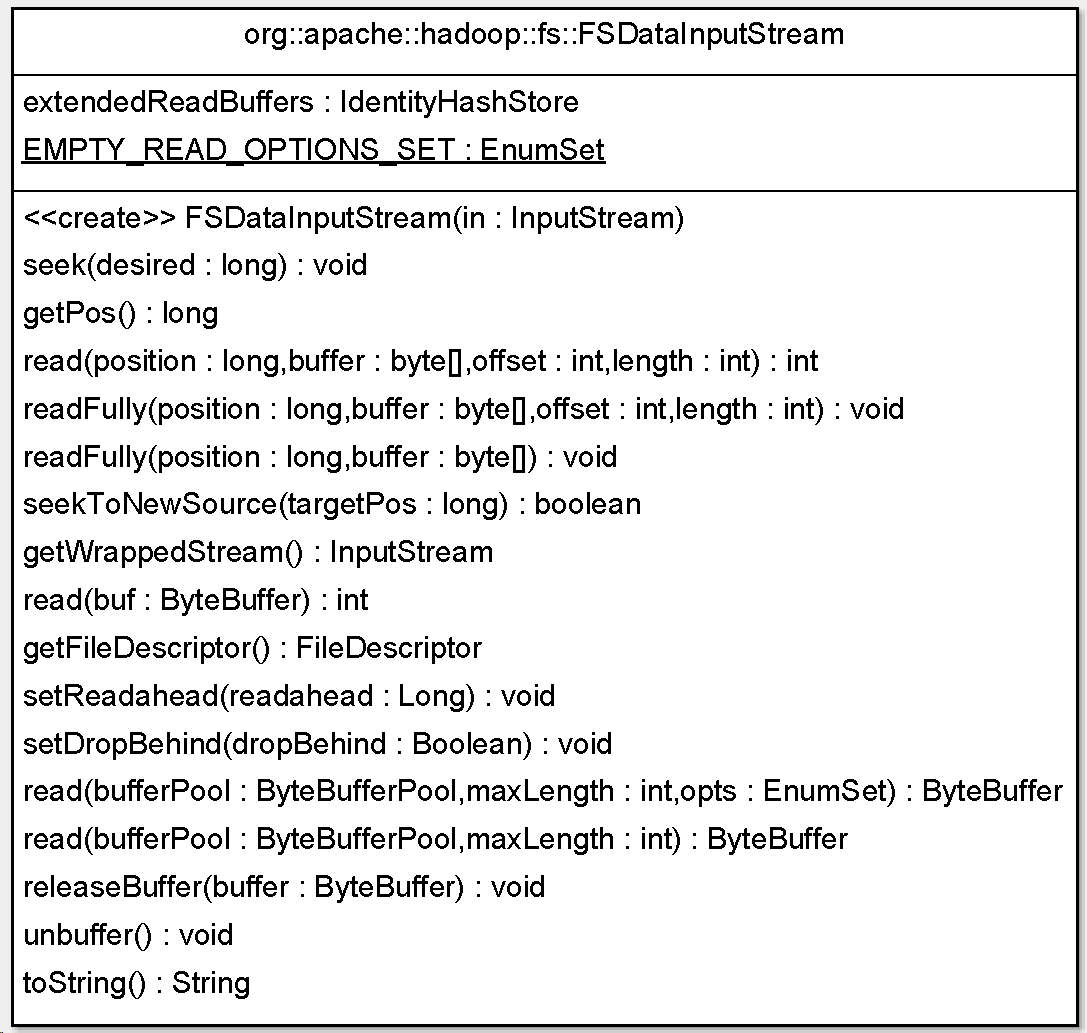
\includegraphics[width=1\linewidth]{fsdatainputstream}
\caption{FSDataInputStream 类的 UML 类图}
\label{fig:fsdatainputstream}
\end{figure}


%% 代码
这个类主要继承于 \lstinline|DataInputStream|,并实现了大量接口
\begin{java}
@InterfaceAudience.Public
@InterfaceStability.Stable
public class FSDataInputStream extends DataInputStream implements Seekable, PositionedReadable, ByteBufferReadable, HasFileDescriptor, CanSetDropBehind, CanSetReadahead, HasEnhancedByteBufferAccess, CanUnbuffer {
\end{java}
构造的方式也和传统的类一样,将\lstinline|InputStream|作为输入参数传入。
\begin{java}
    public FSDataInputStream(InputStream in) {
        /*...*/
    }
\end{java}
实现 \lstinline|Seekable|中的搜索接口,来达到随机读取的目的。
\begin{java}    
    @Override
    public void seek(long desired) throws IOException {
        /*...*/
    }
\end{java}
同时还提供了“定位”的功能,能获得当前位置,完善随机读取的功能。
\begin{java}
    @Override
    public long getPos() throws IOException {
        /*...*/
    }
\end{java}
然后就是大量读取函数的实例了。
\begin{java}    
    @Override
    public int read(long position, byte[] buffer, int offset, int length) throws IOException {
        /*...*/
    }
    
    @Override
    public void readFully(long position, byte[] buffer, int offset, int length) throws IOException {
        /*...*/
    }
    
    @Override
    public void readFully(long position, byte[] buffer) throws IOException {
        /*...*/
    }
    
    @Override
    public int read(ByteBuffer buf) throws IOException {
        /*...*/
    }
    
    @Override
    public ByteBuffer read(ByteBufferPool bufferPool, int maxLength, EnumSet<ReadOption> opts) throws IOException, UnsupportedOperationException {
        /*...*/
    }
\end{code}
此外还提供了一些其他的方法,例如获取文件描述符,缓冲区的操作等。
\begin{code}
    @Override
    public FileDescriptor getFileDescriptor() throws IOException {
        /*...*/
    }

    @Override
    public void setReadahead(Long readahead) throws IOException, UnsupportedOperationException {
        /*...*/
    }
    
    @Override
    public boolean seekToNewSource(long targetPos) throws IOException {
        /*...*/
    }
    
    @InterfaceAudience.LimitedPrivate({"HDFS"})
    public InputStream getWrappedStream() {
        /*...*/
    }

    @Override
    public void setDropBehind(Boolean dropBehind) throws IOException, UnsupportedOperationException {
        /*...*/
    }

    final public ByteBuffer read(ByteBufferPool bufferPool, int maxLength) throws IOException, UnsupportedOperationException {
        /*...*/
    }

    @Override
    public void releaseBuffer(ByteBuffer buffer) {
        /*...*/
    }

    @Override
    public void unbuffer() {
        /*...*/
    }

    @Override
    public String toString() {
        /*...*/
    }
}
\end{java}